\clearpage
\section{Power/Runtime Optimized Software Envelope}

On the nature of software power optimizations... 
We can either reduce activity factor directly or work to tune software to be more dvfs friendly.\todo{Intel energy efficiency optimization guide citation...}

As previously mentioned, only dynamic power consumption may be reduced through code optimizations. \autoref{eq:dynpwr} shows that if an optimization leads to a reduction in activity factor then there will be a corresponding reduction in power consumption. 

\begin{figure}
\centering
\usepgfplotslibrary{fillbetween}

%Fix Area legend to not draw surrounding box
%Taken from http://tex.stackexchange.com/questions/99861/remove-border-around-area-legend-rectangle
\pgfplotsset{
    /pgfplots/area legend/.style={%
        /pgfplots/legend image code/.code={%
            \fill[##1] (0cm,-0.1cm) rectangle (0.6cm,0.1cm);
        }%
    },
}

\begin{tikzpicture}
  \begin{axis}[ticks = none, 
    axis on top,
    axis x line=bottom,
    axis y line=left,
  	xlabel={Runtime \emph{(s)}},
    ylabel={Energy \emph{(J)}},    
    xmin=0, xmax=50,
    ymin=0, ymax=3300,
    width=\linewidth,
    legend style={legend pos=north west}
    ]

    %% Model Parameters %%
    \pgfmathsetmacro{\baselinepower}{30} % NOP code
    \pgfmathsetmacro{\rooflinepower}{60}
    \pgfmathsetmacro{\codepower}{(\baselinepower*3 + \rooflinepower*4) / 7}
    \pgfmathsetmacro{\codetime}{30}
    % Sadly, pgfplots sucks too much to calculate cube roots
    \pgfmathsetmacro{\anodex}{26.20741}
    \pgfmathsetmacro{\anodey}{\anodex * \baselinepower}
    \pgfmathsetmacro{\cnodex}{34.34143}
    \pgfmathsetmacro{\cnodey}{\cnodex * \baselinepower}
    \pgfmathsetmacro{\tnodex}{27.25681}
 
    %% Intermezzo Values %%
    \pgfmathsetmacro{\codeenergy}{\codepower * \codetime}
    \pgfmathsetmacro{\baselineenergy}{\baselinepower * \codetime}
    \pgfmathsetmacro{\rooflineenergy}{\rooflinepower * \codetime}
    \pgfmathsetmacro{\lowdisplayline}{(2 * \baselinepower + \codepower) / 3}
    \pgfmathsetmacro{\highdisplayline}{(1 * \rooflinepower + 1 * \codepower) / 2}
    \pgfmathsetmacro{\rooflinetime}{\codeenergy/\rooflinepower}
    \pgfmathsetmacro{\baselinetime}{\codeenergy/\baselinepower}

    % arguments: code power, code time, x - todo, apparently not supposed to do pgfmathparse
    \pgfmathdeclarefunction{metricbound}{3}{%
      \pgfmathparse{((#1 * #2^3) / #3^2)}%
    }
    \pgfmathdeclarefunction{definitionbound}{3}{%
      \pgfmathparse{((#1 / #2^3) * #3^4)}%
    }
     \pgfmathdeclarefunction{optimizationlimits}{3}{%
      \pgfmathparse{(min(metricbound(#1, #2, #3), definitionbound(#1, #2, #3)))}
    }

    % BETA ROOFLINE BOUND
    \addplot[color=red, name path=roofbound, domain=\pgfkeysvalueof{/pgfplots/xmin}:\pgfkeysvalueof{/pgfplots/xmax}] {\rooflinepower * x};
    \addlegendentry{$P_{max}$ Energy Bound}

    %const power diagonal
    \addplot[color=darkgray, densely dashed, name path=constpwr, forget plot, %forget plot prevents legend entry
            domain=\pgfkeysvalueof{/pgfplots/xmin}:\pgfkeysvalueof{/pgfplots/xmax}] {\codepower * x}; 

    % ALPHA BASELINE BOUND 
    \addplot[color=green, name path=basebound, domain=\pgfkeysvalueof{/pgfplots/xmin}:\pgfkeysvalueof{/pgfplots/xmax}] {\baselinepower * x};
    \addlegendentry{$P_{min}$ Energy Bound} 

    %Runtime Optimization
    \addplot[area legend, fill=blue, fill opacity=0.3, draw=none] coordinates { 
      (\codetime,\rooflineenergy)
      (\codetime,\baselineenergy)
    (0,0)};
    \addlegendentry{Runtime Optimization}

    %Power Optimization
    \addplot[area legend, fill=red, fill opacity=0.2, draw=none] coordinates {
                           (\codetime,\codeenergy)
                           (\pgfkeysvalueof{/pgfplots/xmax},\pgfkeysvalueof{/pgfplots/xmax}*\codepower)
                           (\pgfkeysvalueof{/pgfplots/xmax}, \pgfkeysvalueof{/pgfplots/xmax}*\baselinepower)
                           (0,0)
                         } ;
    \addlegendentry{Power Optimization}
  
    %Energy Optimization
    \addplot[area legend, style={pattern=north west lines, pattern color=gray,
                                 draw=none}] coordinates { 
      (\rooflinetime, \codeenergy)
      (\baselinetime, \codeenergy)
      (0, 0) };
    \addlegendentry{Energy Optimization}



    % Constant Time, Energy Dashes
    %vertical
    \draw[densely dotted] ({axis cs:\codetime,\baselineenergy}) -- ({axis cs:\codetime,\rooflineenergy});
    %horizontal
    \draw[densely dotted, name path=constenergy] ({axis cs:\rooflinetime,\codeenergy}) -- ({axis cs:\baselinetime,\codeenergy});
   

    \node[circle,fill,inner sep=2pt] at (axis cs:\codetime,\codeenergy) {};
    \node[below right] at (axis cs:\codetime,\codeenergy) {$\theta$};


 \end{axis}
\end{tikzpicture}

\caption{Power/Energy/Time tradeoff}
\label{fig:motivation}
\end{figure}

\todo{Different processor subsystems operate at different frequencies. The clock distribution network operates at $\alpha=1$.}
\todo{Clock gating, in which processor elements are isolated from the clock signal and cease to function. When this happens, their activity factor, and hence dynamic power consumption, is zero.}

\todo{reword}
We define the range of values that activity factor can take whilst running a code as $[\alpha  .. \beta]$ where $0 < \alpha < \beta < 1$, and their associated power draws as $P_{\alpha}$ and $P_{\beta}$ respectively, with $P_{\alpha} < P_{\beta}$. By plotting lines with gradients $P_{\alpha}$ and $P_{\beta}$ in \autoref{fig:modeldraw} we establish a feasible performance envelope. This represents the set of all $(E_\theta, D_\theta)$ pairs for which $P_{\alpha}~<~P_\theta~<~P_{\beta}$, with no bounds placed on runtime, $D_\theta$. It should be clear that all code executions, and by extension their maximally-optimized logical equivalents, must be represented somewhere within this envelope. We label the point which corresponds to our original run as $\theta$.
\begin{align}
\frac{{P_{\theta}}^m}{{D_{\theta}}^{m+n}} &= \frac{{P_{\lambda}}^m}{{D_{\lambda}}^{m+n}} \nonumber \\
\implies {P_{\lambda}}^m &= \frac{{P_{\theta}}^m}{{D_{\theta}}^{m+n}} \times {D_\lambda}^{m+n} \nonumber \\ 
\implies {E_{\lambda}}^m &= \frac{{P_{\theta}}^m}{{D_{\theta}}^{m+n}} \times {D_\lambda}^{m+n+1} \nonumber \\ 
\implies E_{\lambda} &= (\frac{{P_{\theta}}^m}{{D_{\theta}}^{m+n}} \times {D_\lambda}^{m+n+1})^{\frac{1}{m}} 
\end{align}

\begin{figure}
\centering
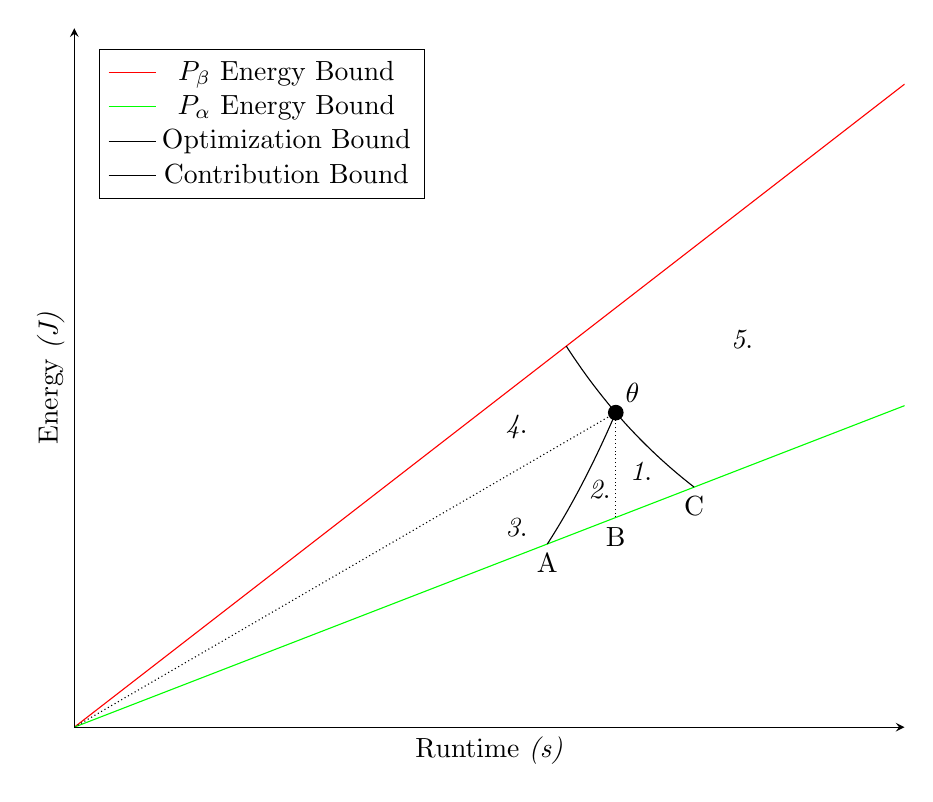
\begin{tikzpicture}

  \begin{axis}[ticks = none, 
    axis on top,
    axis x line=bottom,
    axis y line=left,
	xlabel={Runtime \emph{(s)}},
    ylabel={Energy \emph{(J)}},    
    xmin=0, xmax=46,
    ymin=0, ymax=3000,
    width=\linewidth,
    legend style={legend pos=north west}
    ]

    %% Model Parameters %%
    \pgfmathsetmacro{\baselinepower}{30} % NOP code
    \pgfmathsetmacro{\rooflinepower}{60}
    \pgfmathsetmacro{\codepower}{(\baselinepower + \rooflinepower) / 2}
    \pgfmathsetmacro{\codetime}{30}
    % Sadly, pgfplots sucks too much to calculate cube roots
    \pgfmathsetmacro{\anodex}{26.20741}
    \pgfmathsetmacro{\anodey}{\anodex * \baselinepower}
    \pgfmathsetmacro{\cnodex}{34.34143}
    \pgfmathsetmacro{\cnodey}{\cnodex * \baselinepower}
    \pgfmathsetmacro{\tnodex}{27.25681}
 
    %% Intermezzo Values %%
    \pgfmathsetmacro{\codeenergy}{\codepower * \codetime}
    \pgfmathsetmacro{\baselineenergy}{\baselinepower * \codetime}
    \pgfmathsetmacro{\rooflineenergy}{\rooflinepower * \codetime}
    \pgfmathsetmacro{\lowdisplayline}{(2 * \baselinepower + \codepower) / 3}
    \pgfmathsetmacro{\highdisplayline}{(1 * \rooflinepower + 1 * \codepower) / 2}

    % arguments: code power, code time, x - todo, apparently not supposed to do pgfmathparse
    \pgfmathdeclarefunction{metricbound}{3}{%
      \pgfmathparse{((#1 * #2^3) / #3^2)}%
    }
    \pgfmathdeclarefunction{definitionbound}{3}{%
      \pgfmathparse{((#1 / #2^3) * #3^4)}%
    }
     \pgfmathdeclarefunction{optimizationlimits}{3}{%
      \pgfmathparse{(min(metricbound(#1, #2, #3), definitionbound(#1, #2, #3)))}
    }

    % BETA ROOFLINE BOUND
    \addplot[color=red, name path=roofbound, domain=\pgfkeysvalueof{/pgfplots/xmin}:\pgfkeysvalueof{/pgfplots/xmax}] {\rooflinepower * x};
    \addlegendentry{$P_{\beta}$ Energy Bound}

    % ALPHA BASELINE BOUND 
    \addplot[color=green, name path=basebound, domain=\pgfkeysvalueof{/pgfplots/xmin}:\pgfkeysvalueof{/pgfplots/xmax}] {\baselinepower * x};
    \addlegendentry{$P_{\alpha}$ Energy Bound} 

    % Constant Time and Power Dashes
    \draw[densely dotted] ({axis cs:\codetime,\baselineenergy}) -- ({axis cs:\codetime,\codeenergy});
    \draw[densely dotted] ({axis cs:\pgfkeysvalueof{/pgfplots/xmin},\pgfkeysvalueof{/pgfplots/ymin}}) -- ({axis cs:\codetime,\codeenergy});
 

    \addplot[domain=\tnodex:\cnodex] { metricbound(\codepower, \codetime, x)};
    \addlegendentry{Optimization Bound}

    \addplot[domain=\anodex:\codetime] { definitionbound(\codepower, \codetime, x)};
    \addlegendentry{Contribution Bound}


    \node[circle,fill,inner sep=2pt] at (axis cs:\codetime,\codeenergy) {};
    \node[above right] at (axis cs:\codetime,\codeenergy) {$\theta$};
    \pgfmathsetmacro{\oneycoord}{\lowdisplayline * 31.4}
    \node at (axis cs:31.4,\oneycoord) {\textit1.};
    \pgfmathsetmacro{\twoycoord}{\lowdisplayline * 29.1}
    \node at (axis cs:29.1,\twoycoord) {\textit2.};
    \pgfmathsetmacro{\threeycoord}{\lowdisplayline * 24.5}
    \node at (axis cs:24.5,\threeycoord) {\textit3.};
    \pgfmathsetmacro{\fourycoord}{\highdisplayline * 24.5}
    \node at (axis cs:24.5,\fourycoord) {\textit4.};
    \pgfmathsetmacro{\fiveycoord}{\codepower * 37}
    \node at (axis cs:37,\fiveycoord) {\textit5.};
    
    \node [below] at ({axis cs:\anodex, \anodey}) {A};
    \node [below] at ({axis cs:\codetime,\baselineenergy}) {B};
    \node [below] at ({axis cs:\cnodex, \cnodey}) {C};
    %\node [below, name intersections={of=metric bound and baseline}] at (intersection-1) {C};


 \end{axis}
\end{tikzpicture}

\caption{$ED^2P$ Code Optimization Space}
\label{fig:modeldraw}
\end{figure}
The bounds describe above allow us to identify the area of the Energy/Runtime plane in which power-optimized versions of a given code may exist. We also add lines of constant time and power draw corresponding to the original code for the purpose of illustration. This allows us to subdivide \autoref{fig:modeldraw} into the following labelled areas:
\begin{enumerate}
\item Power-only optimizations
\item Power-mostly optimizations
\item Time-mostly optimizations
\item Time-only optimizations
\item Performance Degradation
\end{enumerate}


\begin{figure}[ht]                                                               
\centering                                                                      
\lstset{basicstyle=\ttfamily\footnotesize\bfseries, frame=tb} %small bold text, lines top and bottom 
\lstinputlisting[]{lst/alpha_benchmark.c}              
\caption{Baseline Power Micro-Benchmark}                            
\label{fig:microbench}                                                           
\end{figure}  
